\documentclass[12pt]{article}
\usepackage[margin=1in]{geometry}
\usepackage{amsmath,amsthm,amssymb}
\usepackage{natbib}
\usepackage{graphicx}
\graphicspath{ {images/} }
 
\newcommand{\N}{\mathbb{N}}
\newcommand{\Z}{\mathbb{Z}}
\newcommand{\R}{\mathbb{R}}
\newcommand{\Indicator}{\mathds{1}}
\newcommand{\EX}{\mathbb{E}}
\newcommand{\Prob}{\mathbb{P}}

\author{Andrew Benton}
\title{Constant bounded approximation algorithms for stochastic inventory control}

\begin{document}

\maketitle

\section{Introduction}

The typical approach for stochastic inventory control models are based on Markov Decision Processes, which are solved through dynamic programming. Although this model is flexible, it can often result in uncomputable solutions. Due to this, there exists a large literature discussing approximation algorithms which are able to compute policies with reasonable efficiency. Unfortunately, understanding the performance of these heuristics can be difficult.\\
\\ 
\cite{levi:2007} present the ideas of \textit{Marginal Cost Accounting} and \textit{Cost Balancing}. Marginal Cost Accounting gives us a method to efficiently compute the full horizon costs incurred by decisions, and thereby avoiding the dynamic programming solution. Cost Balancing allows for an efficient method of solving the resulting equations, and provides bounds on worst case performance. Together, these ideas result in efficient approximation algorithms with bounded worst case performance. 


\subsection{Marginal Cost Accounting}

A cost accounting scheme assigns costs to particular decisions. A marginal cost accounting scheme is one which after a particular decision is made, that cost can be considered to be unalterable by later decisions. Like a myopic policy, marginal cost accounting schemes give us the ability to select optimal decisions in a particular period without any knowledge of later decisions. Unlike a myopic policy, the costs of the decision in future periods are still considered in the current decision. \\
\\
As an example, we consider holding costs. Holding costs have the property that once an order is placed, the holding costs for the particular items purchased will be incurred until they are consumed by demand. Let $h_j$ be the per unit holding cost in period $j$, $D_{[t,j]}$ be the cumulative demand from period $t$ to $j$, and $X_t$ be the inventory in period $t$. The holding costs incurred by an order of size $Q_t$ in period $t$ are:
$$
	\sum_{j=t}^T h_j (Q_t - (D_{[t,j]} - X_t)^+)^+
$$
Note that this equation does not account for any future decisions, allowing the holding costs to be computed for any demand outcome. This allows the expected holding costs to be computed, provided a forecasting distribution over future demands.

\subsection{Cost Balancing}

Cost balancing is the component of the algorithm which provides us with bounded cost guarantees. \cite{levi:2007} provide a detailed proof which the later papers are built upon - only a summary will be offered here. They let $Z_t = \EX[H_t^B \; | \; F_t] = \EX[\Pi_t^B \; | \; F_t]$. They then establish the following equivalency with the total cost of the balancing policy:
$$
	\EX[\mathcal{C}(B)] = 2 \sum_t \EX[Z_t]
$$ 
They then partition the horizon into two sets, $\mathcal{J}_H$ and $\mathcal{J}_{\Pi}$, where inventory held is above and below optimal respectively. Using this partition, they establish that:
$$
	H^{opt} + \Pi^{opt} \geq \sum_{t \in \mathcal{J}_H} H_t^B + \sum_{t \in \mathcal{J}_{\Pi}} \Pi_t^B
$$
With these relationships established, it can be shown that $\EX[\mathcal{C}(opt)] \geq \sum_t \EX[Z_t]$ and therefore:
$$
	\EX[\mathcal{C}(B)] \leq 2 \EX[\mathcal{C}(opt)]
$$
Note that this provides no guarantees about average performance, just worst case performance. \cite{hurley:2007} show that average performance is typically much better, and also provide a set of heuristics for upper and lower bounds for ordering quantity which improve average performance while not violating the constant worst case guarantee. 


\section{Constant Bounded Approximation Algorithms}

\cite{levi:2007} present algorithms for the stochastic inventory control problem and the lot sizing problem. \cite{levi:2008} present algorithms for the capacitated stochastic inventory control problem. \cite{levi:2016} present algorithms for the multi-echelon inventory control problem. For all of these, they present an algorithm as well as worst case performance guarantees. 

\subsection{Stochastic Inventory Problem}

This problem has per unit holding costs $h_s$ and per unit lost sales costs $p_s$. Given the demand sequence $\{z_t\}_t$, a starting inventory $X_t$, the period $s$ holding costs $H^B_s(q_s)$ are computed from the current period to the end of the horizon. 
$$
	H_s^B(q_s) = \sum_{j=s}^T h_j \big[q_s - \big(\sum_{i=s}^j z_i - X_s\big)^+\big]^+
$$
The penalty costs $\Pi_s^B(q_s)$ are simplified by the observation that if too few items are bought during the current period, more can be purchased next period. Due to this, penalty costs only need to be computed for a single period.
$$
	\Pi_s^B(q_s) =  p_s [z_s - (X_s^B + q_s)]^+ 
$$
Using these equations, the Balancing Algorithm seeks the order size $q_s$ where these two costs are equal. That is:
$$
	l_s^B(q_s) = \pi_s^B(q_s)
$$
where $l_s^B(q_s) = \EX[H_s^B(q_s) \; | f_s]$ and $\pi_s^B(q_s) = \EX[\Pi_s^B(q_s) \; | f_s]$. \\
\\
\cite{levi:2007} show that when this $q_s$ is applied, the incurred costs are guaranteed to be twice of the optimal costs. Furthermore, we are provided with two other policies which are known to bound the optimal policy. The first is the Myopic policy, which minimizes only the next period. This is known to overestimate the optimal order quantity. The second is the Minimizing policy, which minimizes the sum of the marginal holding and penalty cost. \cite{levi:2007} show that this overestimates the optimal order quantity. \cite{hurley:2007} show that combining these bounds with the balancing policy, as well as other bounds, provides us with lower cost policy while keeping the worst case guarantees.  

\subsection{Lot Sizing Problem}

This problem has per unit holding costs $h_s$, per unit lost sales costs $p_s$, and a per order fixed cost $K$. The approach taken by Levi et al. (2007) seeks to separately balance the holding costs and ordering costs as well as the penalty costs and ordering costs. Here, the Balancing Algorithm provides two parameters: the inventory level at which to order, and the level to order up to (analagous to (s, S) in the exact formulation of this problem). An order is made if the backordering costs exceed $K$:
$$
	r_s^B = \min_{q} \{q \; : \; \pi_s^B(q_s) \leq K\} 
$$
The order size is then:
$$
	q_s^B = \max_{q_s} \{q \; : \; l_s^B(q_s) \leq K\} 
$$
\cite{levi:2007} show that when this policy is applied, the incurred costs are guaranteed to be three times of the optimal costs. Unfortunately, these bounds assume that the current period's demand is known deterministically. While this is true in some cases, it does limit the applicability.

\subsection{Capacitated Stochastic Inventory Problem}

This problem has per unit holding costs $h_s$, per unit lost sales costs $p_s$, and a maximum order size $u_s$. This problem is effectively a generalization of the uncapacitated stochastic inventory problem, and the balancing algorithm treats it as such. The holding costs are computed the same, but the penalties must now be computed over the whole horizon:
$$
	\tilde{\Pi}(q_s) = \sum_{j=s}^T p_j \big[\big(\sum_{i=s}^j z_i - (q_s + X_s + \sum_{i=s}^j u_i\big)\big)^+ - \big(\sum_{i=s}^j z_i - (q_s + X_s + \sum_{i=s}^j u_i\big)\big)^+\big]
$$
The balancing algorithm then seeks the order size $q_s$ such that:
$$
	l_s^B(q_s) = \tilde{\pi}(q_s)
$$
where $l_s^B(q_s) = \EX[H_s^B(q_s) \; | f_s]$ and $\tilde{\pi}_s^B(q_s) = \EX[\tilde{\Pi}_s^B(q_s) \; | f_s]$. \cite{levi:2008} show that when this $q_s$ is applied, the incurred costs are bounded by two times the optimal costs.

\subsection{Multiechelon Stochastic Inventory Problem}

The final set of models are described by \cite{levi:2016}. The problem requires the presentation of much notation, so full details will be left to the original paper. This paper shows that solving the multiechelon problems with $n$ stages requires solving $n$ separate balancing policies. These balancing policies are similar to the ones seen above, but with extra holding costs accounted for. For the $n$ stage problem, it is shown that the incurred costs are bounded by twice the optimal costs.

\section{Methods for Computing Balancing Policies}

\cite{levi:2007}, \cite{levi:2008}, and \cite{levi:2016} discuss the logic and structure of these algorithms, but offer little advice on how to compute them. \cite{yu:2010} give some detail, but restrict themselves to poisson demand and rely on an graphical method to initialize the algorithm. \cite{hurley:2007} rely on simulation. The following section contains a detailed description of exactly and efficiently computing the balancing policies for independent or multivariate normal demand distributions. 

\subsection{Analysis of Cost Functions}

\subsubsection*{Marginal Holding Cost $l_s^B(q_s)$}

Computing $l_s^B(q_s)$ in the general case requires the computation of a $T - s$ dimensional integral. Traditional cubature algorithms have exponential complexity in dimensions, making such an integral unreasonable to compute. However, some conditions allow it to be reduced to $T-s$ integrals of fewer dimensions. Letting $\Phi$ be the (generally multivariate) distribution of forecast $f_s$: 
\begin{alignat*}{1}
	l_s^B(q_s) &= \EX [H_s^B(q_s) \; | \; f_s] \\
        &= \EX \bigg\{\sum_{j=s}^T h_j\bigg[q_s - \bigg(\sum_{i=s}^j D_i - X_s\bigg)^+\bigg]^+  \; | \; f_s \bigg\} \\
		&= \int_{z_s=0}^{\infty} \int_{z_{(s+1)}=0}^{\infty}\dots \int_{z_T=0}^{\infty}\sum_{j=s}^T h_j\bigg[q_s - \bigg(\sum_{i=s}^j z_i - X_s\bigg)^+\bigg]^+ d\Phi(z_s, z_{s+1}, \dots z_T)
\end{alignat*}
Assuming that the demand of any period would depend only on past demand (rather than future demand), this can be rewritten as a series of $1, 2, \dots, T - s$ dimensional integrals: 
\begin{equation*}
	  l_s^B(q_s) = \sum_{j=s}^T \int_{z_s=0}^{\infty} \int_{z_{(s+1)}=0}^{\infty}\dots \int_{z_j=0}^{\infty} h_j\bigg[q_s - \bigg(\sum_{i=s}^j z_i - X_s\bigg)^+\bigg]^+ d\Phi(z_s, z_{s+1}, \dots z_j)
\end{equation*}
Letting $\psi_{[s,j]}$ be the (possibly uncomputable) distribution function of cumulative demand, $l_s^B(q_s)$ and $\frac{d}{d q_s} l_s^B(q_s)$ can be expressed as $T - s$ integrals in one dimension:
\begin{equation}
	l_s^B(q_s) = \sum_{j=s}^T  h_j \int_{z_j=X_s}^{X_s + q_s}\bigg(q_s + X_s - z_j \bigg) \psi_{[s,j]} (z_j) dz_j
\end{equation}
\begin{equation}
	\frac{d}{d q_s} l_s^B(q_s) =  \sum_{j=s}^T h_j \int_{z_j=X_s}^{X_s + q_s}  \psi_{[s,j]}(z_j) dz_j
\end{equation}
$l_s^B(q_s)$ is convex increasing with $q_s$. For nonincreasing $h_j$, the series in $l_s^B(q_s)$ is nonincreasing with $j$. This allows the series to be truncated with a bounded error. This is particularly useful for dependent demand distributions, as it allows us to compute the expectation over fewer random variables (often only 1 or 2 if $q_s$ is below or near its optimal value). So long as the bounded error is less than the tolerance of the quadrature algorithm, this approximation will result in trivial error, while allowing faster function evaluations.\\
\\
For independent demand, $\psi_{[s,j]} = \phi_s \star \phi_{s+1} \star \dots \star \phi_j$.
For distributions with closed-form convolutions (Normal, Exponential, etc), this can be evaluated efficiently. For dependent demand, specialized methods are necessary. If the demand distribution follows a multivariate normal (or can be approximated by one), $\psi_{[s,j]} = N(\sum_{i=s}^j \mu_i, \sqrt{\sum_{i=s}^{j} \sum_{k=s}^j \sigma_{i,k}^2})$\footnote{This is not true in general for dependent normal random variables. However, it does hold for multivariate normal random variables.}. For other distributions,  \cite{arbenz:2011} provide an algorithm which has superior convergence to Monte Carlo methods for the relevant number of dimensions.

\subsubsection*{Marginal/Forced Backordering Cost $\tilde{\pi}_s^B(q_s)$}

The derivations and discussion seen above apply here as well. The equivalent results follow:
\begin{equation}
	\tilde{\pi}_s^B(q_s) =  \sum_{j=s}^T \int_{z_j= X_s + q_s + \sum_{i=s}^j u_i }^{\infty} p_j\bigg( z_j - X_s - q_s - \sum_{i=s}^j u_i \bigg)  \psi_{[s,j]}(z_j) dz_j
\end{equation}
\begin{equation}
	\frac{d}{d q_s} \tilde{\pi}_s^B(q_s) = - \sum_{j=s}^T p_j \int_{z_j=X_s + q_s + \sum_{i=s}^j u_i }^{\infty}  \psi_{[s,j]}(z_j) dz_j 
\end{equation}

$\tilde{\pi}$ is convex decreasing with $q_s$. For nonincreasing $p_j$, the series in $\tilde{\pi}_s^B(q_s)$ is nonincreasing. 

\subsection{Computing Balancing Quantities}

The balancing policies seek the value $q_s^B$ at which some set of costs are equal to another. For instance, the dual balancing policies seek $q_s^B$ such that:
\begin{equation}
	l_s^B(q_s^B) = \pi_s^B(q_s^B)
\end{equation}
The following will discuss solving equation (5). Adaptations to solve other policies are simple to apply. \\
\\
If the conditions to compute $\psi_{[s, j]}$ are met, we can exactly compute the cost functions. If $l_s^B(q_s)$, $\frac{d}{d q_s} l_s^B(q_s)$, $\tilde{\pi}_s^B(q_s)$, and $\frac{d}{d q_s} \tilde{\pi}_s^B(q_s)$ are decreasing with $j$, they can be efficiently computed, with sublinear time complexity in the horizon length.\footnote{No formal proof can be provided, but logically: Assuming the integration is constant per period, computing the entire horizon will be linear with horizon length. If truncated, then there will be some horizon length which, if increased, no further integrations will be required. The only difficulty here is whether each integration is constant. Under the conditions given, this tends to hold.} \\
\\
\cite{levi:2007} suggests using bisection methods to solve this. However bisection methods have linear convergence, which is quite slow for this problem. Fortunately, under our current assumptions, superior methods can be used. Because $l_s^B(q_s)$ is convex and increasing and $\tilde{\pi}_s^B(q_s)$ is convex and decreasing, (5) has one root, one basin of attraction, no stationary points, and is continuously differentiable. Given these conditions, Newton-Raphson is a better choice. \\
\\
Newton-Raphson begins with an initial estimate $x_0$, and then iterates the following equation:
$$
	x_{n+1} = x_n + \frac{f(x_n)}{f^{\prime}(x_n)}
$$
This is a very standard method - implementations and various modifications are widely available. For the dual balancing policy, $f$ and $f^{\prime}$ would be defined as follows:
$$
	f(x) = l_s^B(x) - \pi_s^B(x) 
$$
$$
	f_s^{\prime}(x) =  \frac{d}{dx} l_s^B(x) - \frac{d}{dx} \pi_s^B(x) 
$$
Newton-Raphson has quadratic convergence, and as result often requires an order of magnitude fewer function evaluations than the bisection. Furthermore, all but the first Newton-Raphson iteration are "very close" to the optimal value, which, as described in Section 3.1, results in faster function evaluation. \\
\\
The only remaining concern when applying Newton-Raphson is the initial estimate $x_0$. Generally, poor initial estimates can cause subquadratic convergence. There is no general answer to this problem, but numerical experience has indicated that these concerns can be ignored with the initial estimate of $x_0 = \mu_s$.

\section{Algorithm Implementation}

The scenario studied here is the simplest case, the unconstrainted stochastic inventory problem. The demand forecast is $NID(1000, 300)$ with a penalty cost of $p_j = 5$ for all $j$ and a holding cost of $h_j = 1$ for all $j$. There are 100 periods in the horizon. These particular demand numbers were selected because the high standard deviation causes longer holding cost evaluations. The truncation error, as well as the tolerance for the quadrature and root-finding algorithms was set to $1*10^{-9}$. Such an error should be trivial in the context of inventory control. The initial guess was equal to the one period demand mean, $x_0 = 1000$. No bounding heuristics will be used here - only the balancing policy is applied. 
\begin{figure}
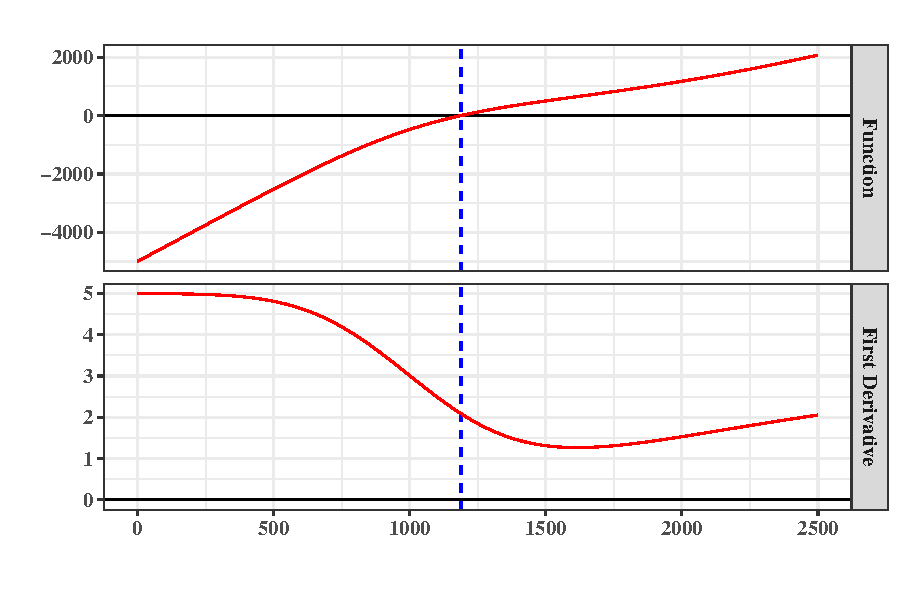
\includegraphics[width=\textwidth]{root_function_report}
\caption{Root function for $NID(1000, 300)$ demand forecasts. Optimal $q$ in blue, $\mu$ in green. The function is generally smooth.}
\end{figure}

\begin{figure}
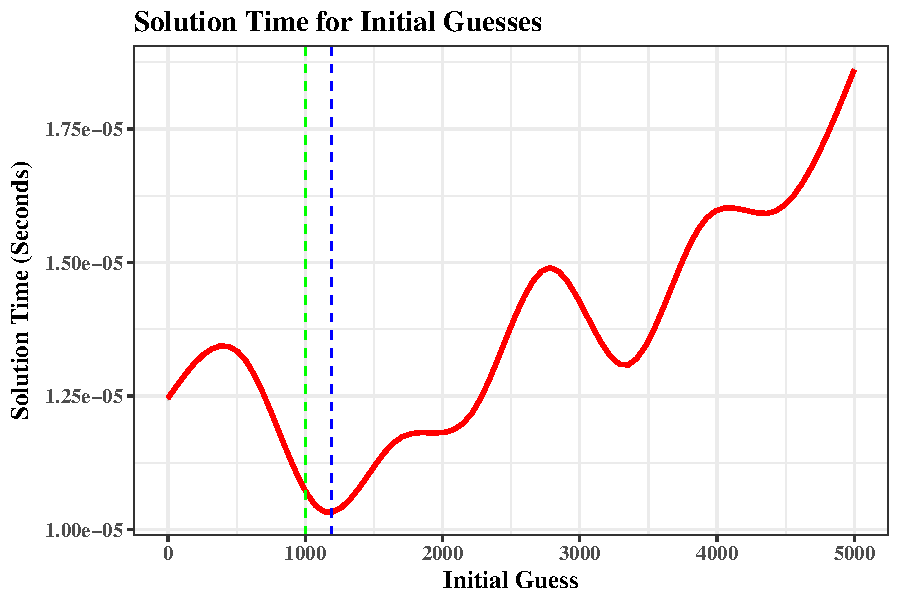
\includegraphics[width=\textwidth]{solution_times_report}
\caption{Solution times plotted for various initial guesses. Optimal $q$ in blue, $\mu$ in green. Although $x_0 = \mu$ is an effective starting point, the running time for any starting point is small.}
\end{figure}
The root function which Newton-Raphson is applied to, as well as the root found by Newton-Raphson, is plotted in Figure 1. Computing this root required 110 nanoseconds. As discussed in section 3.2.1, the solution time depends upon the quality of the initial guess. However, this relationship is plotted in Figure 2, and shows that differences in solution time are trivial in practice. This plot also confirms that the algorithm converges for a wide range of initial guesses ($x_0 \in \{0, 5000\}$ in this case).

\bibliography{citations}
\bibliographystyle{plainnat}

\end{document}
